The normalized chimera-like index of the entire physical region is shown in \cref{fig:aphysical_chimera}.
Near the maximal edge of the physical region, the highest values of the chimera index appear to follow a slope of $-1$.
It is unsurprising that chimera states would be prevalent when the coupling is large (out near the boundary of the aphysical range).
\begin{figure}[ht]
  \centering
  \includegraphics{figure/zoom_chimera}
  \caption[Zoomed landscape]{The chimera index of runs with $(\hra, \hrb) \in (0, 0.2) \times (0, 0.1)$.}
  \label{fig:zoom_chimera}
\end{figure}

What is surprising, however, is the presence of the chimeric patch in the bottom left corner of \cref{fig:aphysical_chimera}, shown at a higher resolution in \cref{fig:zoom_chimera}.
Plotting the results of the simulations (\cref{fig:mean_058_010,fig:overhead_058_010}),
it is evident that this is not a calculation error, but is an actual feature of the parameter landscape.
\todo{Figure out what the heck is going on here.}
\todo{Fix the size and x-scale.}
\begin{figure}[ht]
  \centering
  \begin{subfigure}{\textwidth}
    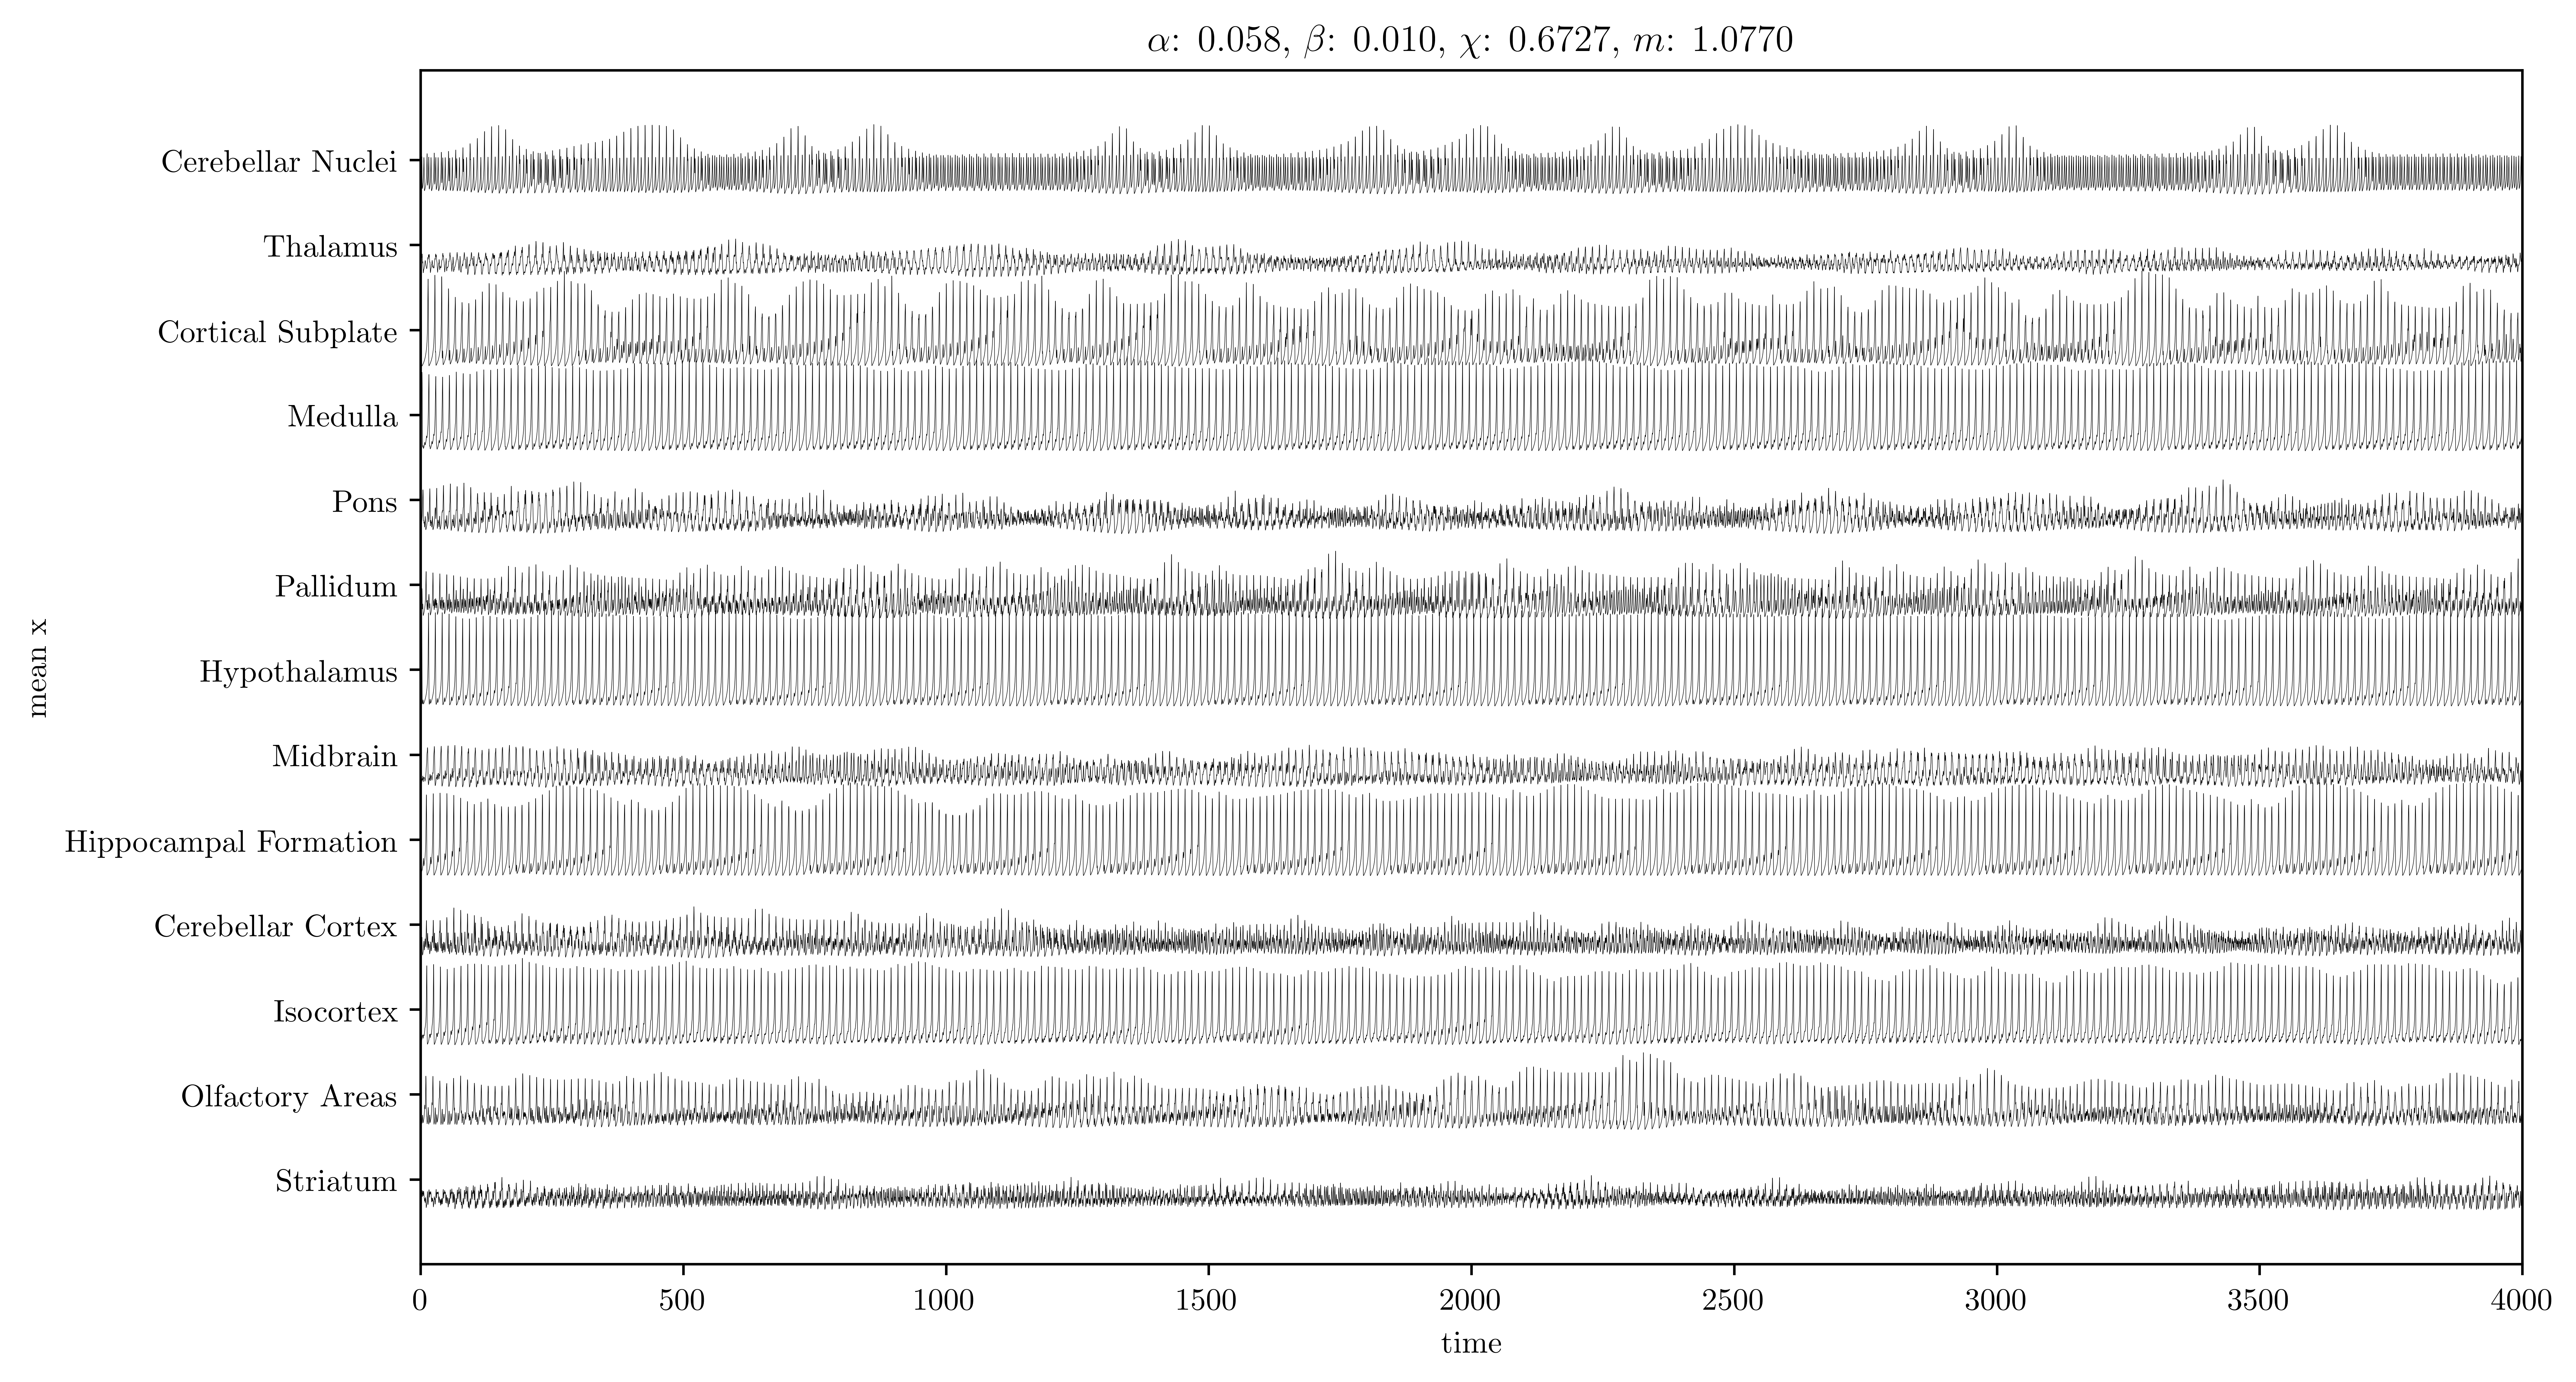
\includegraphics[width=\textwidth]{figure/means-0_058-0_010}
    \caption{The mean membrane potential within each cortex.}
    \label{fig:mean_058_010}
  \end{subfigure}
  \begin{subfigure}{\textwidth}
    \includegraphics[width=\textwidth]{figure/overhead-0_058-0_010}
    \caption{The phase $\phase$ of the entire timeseries for a simulation of the Hindmarsh-Rose network.}
    \label{fig:overhead_058_010}
  \end{subfigure}
  \caption[Highly chimeric simulation]{A run of the Hindmarsh-Rose simulation in the chimeric island.}
  \label{fig:058_010}
\end{figure}

%%% Local Variables:
%%% mode: latex
%%% TeX-master: "../../main"
%%% End:
